\documentclass{article}
\usepackage[utf8]{inputenc}
\usepackage[margin=1in]{geometry}
\usepackage{amsmath, amsfonts}
\usepackage{fancyhdr}
\usepackage{multicol}
\usepackage{graphicx}
\usepackage{amsthm}
\usepackage{pgfplotstable}
\usepackage{longtable}
\usepackage{algorithm2e}
\graphicspath{ {images/} }
\pagestyle{empty}
\fancyhf{}
\cfoot{\thepage}

\newtheorem*{lemma}{Lemma}
\newtheorem*{theorem}{Theorem}
\newcommand{\twonorm}[1]{\| #1 \|_2}
\newcommand{\rdim}[2]{\mathbb{R}^{#1 \times #2}}
\newcommand{\R}{\mathbb{R}}
\lhead{CSCD37: Assignment \#2 }
\rhead{
Poon, Keegan\\
poonkeeg\\
1002423727}
\pagenumbering{gobble}
\renewcommand{\headrulewidth}{0pt}
\begin{document}

\thispagestyle{fancy}
\begin{enumerate}
    \item Recall the full-Newton algorithm for solving the nonlinear system $F(x) = 0; F,x\in \mathcal{R}^n:$

        \begin{algorithm}[H]
            \SetAlgoNoLine
            \SetEndCharOfAlgoLine{}
            \SetKwProg{Fn}{}{}{}
            \Fn{}{
                Generate an initial approximation $\hat x_0$ \;
                for $k = 0,1\dots$ until convergence\;
                \Indp compute $-F(\hat x_k)$ \;
                    compute $\frac{\partial F(\hat x_k)}{\partial x}$ \;
                    solve $\frac{\partial F(\hat x_k)}{\partial x} \Delta_k = -F(\hat x_k)$ \;
                    update $\hat x_{k+1} = \hat x_k + \Delta_k$ \;
                \Indm end for
            }
        \end{algorithm}
        \begin{enumerate}
            \item This algorithm is computationally expensive. Give a detailed analysis of the cost using standard big-oh notation. You may use results from CSCC37; e.e., the cost (measuring flops) of the LU-factorization of an $n \times n$ matrix is $(1/3)n^3 + \mathcal O (n^2)$.

                The following analysis makes the assumption that each component of $F$ can be evaluated in approx 1 flop, and that taking the derivative also takes around 1 flop. For each iteration of the loop, first evaluating the function $F$ at a point $x \in \mathcal{R}^n$ will take n operations. The evaluation of the $n$ derivatives will also take $n$, so evaluating $n$ derivatives at $n$ points will take $n^2$ time. Solving the linear system of the derivative matrix against the original function will take around $(1/3)n^3 + \mathcal{O}(n^2)$ as was seen in CSCC37. Finally updating a vector with an addition of 2 $n$ length vectors will simply be $n$ additions. Overall, the entire loop iteration will take $n^2 + n + (1/3)n^3 + \mathcal{O}(n^2) + n = (1/3)n^3 + \mathcal{O}(n^2) = \mathcal{O}(n^3)$ steps per iteration. This cannot be generalized outside of iterations, as convergence is not always guaranteed and $k$ may run on infinitely.
            \item We briefly discussed in lecture the ``quasi-Newton algorithm" for solvling nonlinear systems. Modify the algorithm above to take advantage of the optimizations we discussed. You do not need to implement the modifications \dots pseudo-code will suffice. Be careful to discuss both flop optimizations and convergence issues (``X-test" and ``F-test" tolerance, maximum number of iterations, condition of Jacobian, how long to hold Jacobian fixed, etc.).
        \end{enumerate}
    \newpage
    \item In lecture we derived the divided-difference (Newton) form of the interpolating polynomial for the simple interpolation problem. This question will investigate how the Newton polynomial can be used for osculatory interpolation.
        \begin{enumerate}
            \item Prove that
                \[ \lim_{\substack{x_{i+j} \rightarrow x_i \\ 1 \leq j \leq k}}y[x_{i+k},x_{i+k-1},\dots,x_i] = \frac{y^{(k)}(x_i)}{k!} \]
                Provided $y \in \mathcal C^k$.

                \begin{proof}
                    Examine first, the error formula given in lecture, $E(x) = y(x) - p(x)$ for any polynomial interpolant, then using the Newton polynomial as $p(x)$, it produces:
                    \[ E(x) = y(x) - y[x_i] + (x-x_i)y[x_{i+1},x_i] + \cdots + (x - x_i)(x - x_{i+1}) \cdots(x - x_{i + k-1})y[x_{i + k},\dots,x_i]\]
                    Knowing that $E(x)$ has $n+1$ distinct roots (at the interpolation constraints), by Rolle's theorem, gives that the $k$th derivative of $E(x)$ has at least 1 zero $E(\psi)$ where $\psi \in$ span$\{x_i,\dots,x_{i+k}\}$. Looking at the Newton polynomial, the $k$th derivative will only have the leading coefficient times $k!$ since it is a degree $k$ polynomial. This coefficient, from the definition can be seen as $y[x_{i+k},\dots,x_i]$
                    \begin{align*} 
                        \implies \frac{d^k}{dx^k} E(x) &= y^{(k)}(x) - y[x_{i+k},\dots,x_i]k!  \\
                        \frac{d^k}{dx^k} E(\psi) &= y^{(k)}(\psi) - y[x_{i+k},\dots,x_i]k!  \\
                        0 &= y^{(k)}(\psi) - y[x_{i+k},\dots,x_i]k!  \\
                        y[x_{i+k},\dots,x_i]k! &= y^{(k)}(\psi) \\
                        y[x_{i+k},\dots,x_i] &= \frac{y^{(k)}(\psi)}{k!} \\
                        \implies \lim_{\substack{x_{i+j} \rightarrow x_i \\ 1 \leq j \leq k}} y[x_{i+k},\dots,x_i] &= \lim_{\substack{x_{i+j} \rightarrow x_i \\ 1 \leq j \leq k}} \frac{y^{(k)}(\psi)}{k!} \\
                        \implies \lim_{\substack{x_{i+j} \rightarrow x_i \\ 1 \leq j \leq k}} y[x_{i+k},\dots,x_i] &= \frac{y^{(k)}(x_i)}{k!} \\
                    \end{align*}
                    The last line is since if $\forall x_{i+j},\, |x_{i+j} - x_i| < \varepsilon \implies$ span$\{x_i,\dots,x_{i+k}\} \subset (x_i - \varepsilon,\, x_i + \varepsilon) \implies \psi \rightarrow x_i$.

                \end{proof}   
            \item The result in (a) tells us that divided differences can be replaced with derivatives as data points coincide. Using this result, construct a divided difference table to find the coefficients of the Newton polynomial of degree 6 or less that satisfies the following interpolation conditions:
                \begin{align*}
                    &p(-1) = 4& &p(0) = 7& &p(1) = 28& &p(2) = 247& \\
                    & & &p'(0) = 6& &p'(1) = 56& & & \\
                    & & & & &p''(1) = 140& & & \\
                \end{align*}
                \[
                \begin{array}{cccccccc}
                x_0 & y(x_0) \\
                    &         & y[x_1,x_0] \\
                x_1 & y(x_1)  &             & y[x_1,x_1,x_0]\\
                    &         & y[x_1,x_1]  &                & y[x_2,x_1,x_1,x_0]\\
                x_1 & y(x_1)  &             & y[x_2,x_1,x_1] &                    & y[x_2,x_2,x_1,x_1, x_0]\\
                    &         & y[x_2,x_1]  &                & y[x_2,x_2,x_1,x_1] &                         & y[x_2,x_2,x_2,x_1,x_1, x_0]  \\
                x_2 & y(x_2)  &             & y[x_2,x_2,x_1] &                    & y[x_2,x_2,x_2,x_1, x_1] &               & y[x_3, \dots x_0]\\
                    &         & y[x_2,x_2]  &                & y[x_2,x_2,x_2,x_1] &                         & y[x_3,x_2,x_2,x_2,x_1, x_1] \\
                x_2 & y(x_2)  &             & y[x_2,x_2,x_2] &                    & y[x_3,x_2,x_2,x_2, x_1]\\
                    &         & y[x_2,x_2]  &                & y[x_3,x_2,x_2,x_2]\\
                x_2 & y(x_2)  &             & y[x_3,x_2,x_2]\\
                    &         & y[x_3,x_2] \\
                x_3 & y(x_3)  &  
                \end{array}
                \]
                \[
                \begin{array}{cccccccc}
                -1  & 4   \\
                    &      & 3          \\
                0   & 7    &             & 3           \\
                    &      & 6           &              & 6          \\
                0   & 7    &             & 15           &             & 7           \\
                    &      & 21          &              & 20          &              & 4            \\
                1   & 28   &             & 35           &             & 15           &               &  1           \\
                    &      & 56          &              & 35          &              & 7            \\
                1   & 28   &             & 70           &             & 29          \\
                    &      & 56          &              & 93         \\
                1   & 28   &             & 163         \\ 
                    &      & 219        \\
                2   & 247  &  
                \end{array}
                \]
            \[ \implies p(x) = 4 + 3(x+1) + 3(x+1)x + 6(x+1)x^2 + 7(x+1)x^2(x-1) + 4(x+1)x^2(x-1)^2 + (x+1)x^2(x-1)^3 \]
            \[ \iff p(x) = x^6 + 2x^5 + 3x^4 + 4x^3 + 5x^2 + 6x + 7 \]
            \item Use the Method of Undetermined Coefficients (i.e., as discussed in lecture, construct and solve an appropriate Vandermonde system) to find the coefficients of the monomial-basis polynomial of degree 6 or less that satisfies the interpolation conditions specified in (b).
                You may use \textit{MatLab} for this question if you wish. Verify that you have obtained the same polynomial as in (b).
                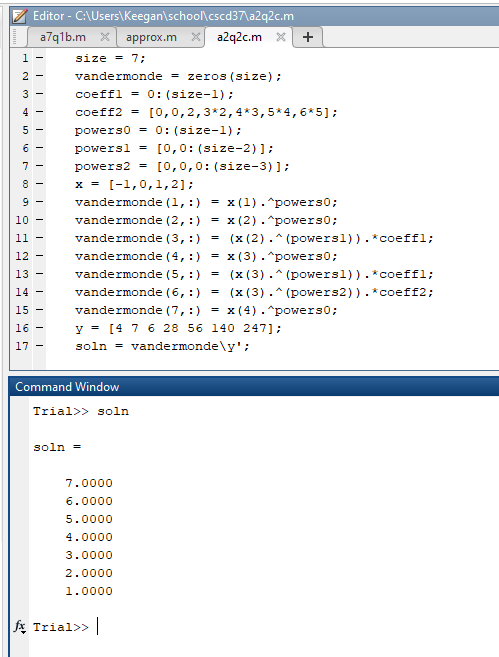
\includegraphics{a2-q2-c}
        \end{enumerate}
    \newpage
    \item Consider the function $y\in \mathcal C^{n+1}$ and the polynomial $p \in \mathcal P_n$ which satisfies
        \[ p^{(j)}(x_i) = y^{(j)}(x_i); \; j=0,\dots,j_i; \; i=0,\dots,k; \; \sum_{i=0}^k (j_i + 1) = n+1;\]
        with all of the $x_i$ distinct. The error in this polynomial interpolant is given by
        \begin{equation}
            E(x) = y(x) - p(x) = \frac{y^{(n+1)}(\xi)}{(n+1)!} (x-x_0)^{j_0+1}(x-x_1)^{j_1+1}\cdots(x-x_k)^{j_k+1}
        \end{equation}
        where $\xi \in $ span$\{x_0,\dots,x_k,x\}$ = $[\min\{x_0,\dots,x_k,x\},\max\{x_0,\dots,x_k,x\}]$ provided $y \in \mathcal C^{n+1}$ on span$\{x_0,\dots,x_k,x\}$.

        This is a fundemental formula in Numerical Aprroximation. The following is an outline of a possible derivation of (1). In this question you will expand this outline by proving certain key statements.

        If $x = x_i,\, i=0,\dots,k,$ then $y(x)-p(x) = 0$ since $p$ interpolates $y$ at these $k+1$ points. Also, $E(x_i) = 0$ in (1) since $(x_i-x_i)^{j_1+1} = 0$. Therefore, (1) holds when $x=x_i$.
        
        Now assume $x \not = x_i$ for any $i = 0,\dots,k$ and consider $x$ \textit{fixed}. Let $F(t) = y(t) - p(t) - CW(t)$ where $C = [y(x) - p(x)]/W(x)$ is a constant and
        \begin{equation}
            W(t) = (t-x_0)^{j_0 +1}(t-x_1)^{j_1+1}\cdots (t-x_k)^{j_k+1}
        \end{equation}
        is a polynomial of degree $n+1$. Clearly $F(x) = 0$, and also
        \begin{equation}
            F^{(j)}(x_i) = 0;\; j=0,\dots,j_i;\; i=0,\dots,k.
        \end{equation}

        Therefore, counting multiplicities, $F(t)$ has at least $n+2$ zeros in span$\{x_0,\dots,x_k,x\}$, which implies $F^{(n+1)}(t)$ has at least 1 zero in span$\{x_0,\dots,x_k,x\}$, or, in other words,

        \begin{equation}
            F^{(n+1)}(\xi) = 0, \xi \in \text{span}\{x_0,\dots,x_k,x\}.
        \end{equation}
        But

        \begin{equation}
            F^{(n+1)}(t) = \frac{d^{n+1}}{dt^{n+1}}[y(t) - p(t) - CW(t)] = y^{(n+1)}(t) - (n+1)!C.
        \end{equation}

        Therefore,
            \[ F^{(n+1)}(\xi) = 0 \implies y^{(n+1)}(\xi) - (n+1)!C = 0 \implies C = \frac{y^{(n+1)}(\xi)}{(n+1)!}. \] 
        But
            \[ C = \frac{y(x) - p(x)}{W(x)} \implies y(x) - p(x) = \frac{y^{(n+1)}(\xi)}{(n+1)!}W(x). \]
        Now for the statements you must prove:
        \begin{enumerate}
            \item Prove that $W(t)$ in (2) is a polynomial of degree $n+1$.
                \begin{proof}
                Polynomials are closed under exponentiation and basic operations, so it is sufficient to show the highest power to be $n+1$. For each term $(t - x_i)^{j_i + 1}$, the highest power of $t$ is $j_i + 1$ respectively using the Binomial Theorem. This means that the final product will highest power of all of these terms together, so the power will be $\sum_{i=0}^{k}j_i + 1 = n + 1$ by definition.
                \end{proof}
            \item Prove (3)
                \begin{proof}
                    We know that $p$ must approximate $y$ exactly at the interpolation points, so evidently for a point on the $j$th derivative, $y^{(j)}(x_i) - p^{(j)}(x_i)$ will be 0. For the other term $CW(t)$, taking the derivative only $j$ times will result in the term $(x - x_i)$ to show up in every term generated by the product rule since it has power of $(j_i + 1)$, hence $W(t)$ will also be 0 making $F^{(j)}(x_i) = 0$ at all interpolation points.
                \end{proof}
            \item Explain how (4) follows from $F(t)$ having at least $n+2$ zeros in span$\{x_0,\dots,x_k\}$.
                \begin{lemma}
                    Counting multiplicities, if $F(t)$ is $\mathcal C^1$ over span$\{x_0,\dots,x_k\}$ has at least $k$ zeros in span$\{x_0,\dots,x_k\}$ then $F'(t)$ has at least $k-1$ zeros in span$\{x_0,\dots,x_k\}$.
                \end{lemma}
                \begin{proof}
                    Suppose the distinct roots of $F(t)$ are ordered as $a_1 < a_2 < \cdots < a_s$ with multiplicities $m(a_i)$ such that $\sum_{i=0}^s m(a_i) = n$. From Rolle's Theorem, we have that there is some $\rho \in (a_i, a_{i+1}),\: 1\leq i < s$ where $F'(\rho) = 0$ immediately giving us $s - 1$ roots in the derivative. Now counting the multiplicities of the previous roots, we get that there are $\sum_{i=0}^s (m(a_i) - 1)$ more roots, which summing together gives $\sum_{i=0}^s m(a_i) - s + (s - 1) = n - 1$ roots, which are all in the span.
                \end{proof} 
                From this, it follows immediately that taking $n+1$ derivatives of a function with $n+2$ roots will have one root in the same span.
            \item Prove (5).
                \begin{proof}
                    Since $p$ is a polynomial of degree $n$, taking $n+1$ derivatives will immediately cause it to vanish. On the otherhand, for $W(t)$, we know it is a polynomial of degree $n+1$ from (a), so taking the $(n+1)$th derivative gives us the leading coefficient times $(n+1)!$. Looking back at how $W(t)$ is setup though, since none of the $t$ in each binomial term have any coefficient the resulting expanded polynomials leading coefficient will be 1. This means the $(n+1)$th derivative of $CW(t)$ is just $C(n+1)!$.
                    \begin{align*} 
                        \implies F^{(n+1)}(t) &= \frac{d^{n+1}}{dt^{n+1}}[y(t) - p(t) - CW(t)] \\
                        &= \frac{d^{n+1}}{dt^{n+1}}y(t) - \frac{d^{n+1}}{dt^{n+1}}p(t) - \frac{d^{n+1}}{dt^{n+1}}CW(t)  \\
                        &= y^{(n+1)}(t) - (n+1)!C.
                    \end{align*}
                \end{proof}  
        \end{enumerate}
    \newpage
    \item In lecture we proved that the roots of the Chebyshev polynomial
        \begin{equation}
            T_k(x) = \cos(k\cos^{-1}(x)), k=0,1,\dots
        \end{equation}
        are the optimal interpolation points on [-1,1].
        \begin{enumerate}
            \item Prove that (6) is a polynomial of degree $k$ for all $k \geq 0$.
                \begin{proof}
                    For the case of $k= 0,  1$, we have that 
                    \begin{align*}
                        \cos(k\arccos(x)) |_{k=0} &= \cos(0) = 1 \\
                        \cos(k\arccos(x)) |_{k=1} &= \cos(\arccos x) = x \\
                    \end{align*}
                    So these cases hold. Using induction, assume that $T_n(x)$ is a polynomial for $n < k$, then there are two inductive cases:

                    First $k = 2t$ is even
                    \begin{align*}
                        \cos(k\arccos(x)) &= \cos(2(t\arccos(x)))  \\
                        &= 2(\cos(t\arccos(x)))^2 - 1 \text{ [Double angle identity]}\\
                        &= 2(T_t(x))^2 - 1 
                    \end{align*}
                    This is again a polynomial since $T_t$ is one by IH, so this case holds.

                    Second $k = 2t + 1$ is odd
                    \begin{align*}
                        \cos(k\arccos(x)) &= \cos(2(t\arccos(x)) + \arccos(x)) \\
                        &\overset{\text{angle sum}}{=} \cos(2t\arccos(x))(\cos(\arccos(x))) - \sin(2t\arccos(x))(\sin(\arccos(x))) \\
                        &= xT_{2t}(x)- \sin(2t\arccos(x))(\sin(\arccos(x))) \\
                        &\overset{\text{double angle}}{=} xT_{2k}(x)- 2\cos(t\arccos(x))\sin(t\arccos(x))(\sin(\arccos(x))) \\
                        &= xT_{2t}(x)- 2T_t(x)\sin(t\arccos(x))(\sin(\arccos(x))) \\
                        &\overset{\text{angle prod}}{=} xT_{2k}(x)- T_t(x)(\cos((t-1)\arccos(x))-\cos((t+1)\arccos(x)))\\
                        &= xT_{2t}(x)- T_t(x)(T_{t-1}-T_{t+1})\\
                    \end{align*}
                    Which is again a polynomial all the lower degrees of $T$ are polynomials by IH, so both cases hold.
                \end{proof}
            \item Derive the leading coefficient of (6) (i.e., the coefficient of $x^k$).

                The coefficient is $2^{k-1}$ for $k \geq 1$ and $1$ for $k=0$.
                \begin{proof}
                    Again, using induction, the case of $1$ and $0$ are trivial, as $T_0(x) = 1$ and $T_1(x) = x$. For the inductive case, consider again even and odd, and assume that it holds for $n < k$.

                    For $k = 2t$ even, the leading coefficient $\mathcal L \mathcal C (T_k)$:
                    \begin{align*}
                        \mathcal L \mathcal C (T_k) &= 2 \mathcal L \mathcal C (T_t)^2 \text{ From the recurrence in (a)} \\
                        &= 2  (2^{t-1})^2 = 2 (2^{2t-2}) = 2^{k-1} \text{ By IH}\\
                    \end{align*}

                    For $k = 2t+1$ odd,
                    \begin{align*}
                        \mathcal L \mathcal C (T_k) &= \mathcal L \mathcal C (T_{k-1}) + \mathcal L \mathcal C (T_t) \mathcal L \mathcal C (T_{t+1}) \text{ From the other recurrence in (a)} \\
                        &= 2^{k-2} + (2^{t-1})(2^t) \text{ From IH} \\
                        &= 2^{k-2} + 2^{2t-1}\\
                        &= 2^{k-2} + 2^{k-2} = 2^{k-1}\\
                    \end{align*}

                \end{proof} 
            \item Derive the roots of (6) (i.e., the so-called Chebyshev points).
                
                The roots for a polynomial of degree $k$ are $x_i = \cos(\frac{(2i+1)\pi}{2k})$ where $i = 0,\dots k-1$.
                \begin{proof}
                    Given the definition for $T_k$, plugging in $x_i$ gives
                    \begin{align*}
                        \cos(k\arccos(x_i)) &= \cos(k\arccos (\cos\Big(\frac{(2i+1)\pi}{2k}\Big))) \\
                        &= \cos\Big(k\frac{(2i+1)\pi}{2k}\Big) \\
                        &= \cos\Big(\frac{(2i+1)\pi}{2}\Big) \\
                        &= 0 \, \text{ When }i \in \mathbb{N}
                    \end{align*} 
                \end{proof}  
            \item Complete the proof showing why the Chebyshev points are optimal.

            Since the Chebyshev polynomial is infact a polynomial, with coefficient $2^{k-1}$, we can write it out as $2^{k-1}(x-x_1)(x-x_2)\cdots(x-x_k)$, where $x_i,\, 1\leq i \leq k$ are the roots of $x_i$. It can also be converted to a monic polyomial by dividing by $2^{k-1}$. Note that it is also bound between -1 and 1 because of the $\cos$ definition of $T_k$ To show that they are optimal, we prove the following:
            \begin{theorem}
                If W(x) is a monic polynomial of degree $\leq k$, then $\displaystyle \max_{x} |W(x)| \geq \max_{x} \Big| \frac{T_k(x)}{2^{k-1}}\Big| = \frac{1}{2^{k-1}}$
            \end{theorem}
            \begin{proof}
                Suppose $\displaystyle \max_{x} |W(x)| < \max_{x} \Big| \frac{T_k(x)}{2^{k-1}}\Big|$, then in particular $|W(y_i)| < \Big| \frac{T_k(y_i)}{2^{k-1}}\Big| = \frac{1}{2^{k-1}}$ where $y_i = \cos(\frac{i\pi}{k})$ since looking at the definition of $T_k$ these are the absolute maximums, specifically
                \[
                    T_k(y_i) =
                    \begin{cases}
                         1 & i \text{ even} \\
                        -1 & i \text{ odd} \\
                    \end{cases}
                \]
            \end{proof}
            Now consider the polynomial $q(x) = \frac{T_k(x)}{2^{k-1}} - W(x)$ which is in $\mathcal{P}_{k-1}$ since both polynomials are monic, hence the highest power will cancel. Now look at what happens in the case of plugging in $y_i$. So 
            \[ q(y_i) = \frac{T_k(y_i)}{2^{k-1}} - W(y_i)
                = \begin{cases}
                    > 0 & i \text{ even} \\
                    < 0 & i \text{ odd}
                  \end{cases}
                  \]
            This is the case, since at even points $T_k$ is positive, and the absolute value of $W$ is less then $T_k/2^{k-1}$ so it could not possibly subtract more then 1. Likewise for the $i$ odd case it cannot add enough since the absolute value is less than $T_k/2^{k-1}$. This means that $q(x)$ has a root in each interval $[y_i,\, y_{i+1}]$ for $i=0,\dots,k-1$ so $q$ has $k$ roots, but $q \in \mathcal{P}_{k-1}$ so $q = 0$, so $\frac{T_k(x)}{2^{k-1}} - W(x) = 0$, which is a contradiction to our assumption. Hence, $\frac{T_k(x)}{2^{k-1}}$ is the smallest possible polynomial that $W$ could be, so using the Chebyshev points will make $W$ optimal.
        

        \end{enumerate}
    \newpage
    \item Consider the definite integral $I(f) = \int_{-1}^1 f(x) \,dx$.

        \begin{enumerate}
            \item Construct the interpolatory quadrature rule for this integral based on nodes $-1, -\frac{1}{2}, \frac{1}{2}, 1$.

            \[p(x) = \sum_{i=0}^n f(x_i)l_i(x),\; p(x) \in \mathcal{P}_n\]
            \[l_i = \prod_{\substack{j=1 \\ j\neq i}}^n\frac{x-x_j}{x_i-x_j} \]
            \begin{align*}
                l_1 &= \Big( \frac{x - x_2}{x_1 - x_2}\Big)\Big( \frac{x - x_3}{x_1 - x_3}\Big)\Big( \frac{x - x_4}{x_1 - x_4}\Big)\\ 
                &= \Big( \frac{x - -1/2}{x_1 - -1/2}\Big)\Big( \frac{x - x_3}{x_1 - x_3}\Big)\Big( \frac{x - x_4}{x_1 - x_4}\Big)\\ 
                l_2 &= \prod_{\substack{j=1 \\ j\neq i}}^n\frac{x-x_j}{x_i-x_j} \\
                l_3 &= \prod_{\substack{j=1 \\ j\neq i}}^n\frac{x-x_j}{x_i-x_j} \\
                l_4 &= \prod_{\substack{j=1 \\ j\neq i}}^n\frac{x-x_j}{x_i-x_j} \\
            \end{align*}

            \item What is the precision of the quadrature rule derived in (a)? \textbf{Justify your answer.}
            \item Find as good an error bound as you can for your quadrature rule, assuming $f$ is as smooth as required for your analysis.
        \end{enumerate}
\end{enumerate}
\end{document}
